\documentclass[english]{../thermomemo/thermomemo}
%
\usepackage{lastpage}
\usepackage{amsmath, amssymb, amsthm}
\usepackage{pifont}
\usepackage{moreverb}
\usepackage[latin1]{inputenc}
%\usepackage[T1]{fontenc}
\usepackage{verbatim}
\usepackage{ae, aecompl}
\usepackage[british]{babel}
\usepackage{appendix}
\usepackage{cite}
\usepackage{xcolor}
\hypersetup{
    colorlinks,
    linkcolor={red!50!black},
    citecolor={blue!50!black},
    urlcolor={blue!80!black}
}
\newcommand*{\X}{\ding{51}}
\title{Flexible thermodynamic workbench for CCS thermodynamics}
\author{\O{ivind} Wilhelmsen, Geir Skaugen and Morten Hammer}
\date{2013-11-20}
\begin{document}

\frontmatter
\tableofcontents

\graphicspath{{gfx/}}

\section{Introduction}
In the project CO$_2$ Dynamics, the overall aim is to provide knowledge about
safe and efficient design and operation of CO$_2$-pipeline transport and
injection systems. To achieve this, knowledge about the thermo-physical
properties of CO$_2$-mixtures is needed. Thermo-physical properties can be
densities, viscosities, heat capacities and much more. Since these are
necessary input to all higher level modeling, accurate, robust and fast
theoretical models are prerequisites for reliable process and scenario
evaluations. CO$_2$-Dynamics started already in 2009. In 2009 and 2010,
in-house thermodynamic routines were tested and used to do regression of
interaction parameters for cubic equations of state capable of handling CO$_2$
mixtures. This was documented in the memo DA1001. In 2011, other equations of
state such as Lee-Kesler and the SPUNG approach were tested for
CO$_2$-mixtures and presented in a paper (DA1103). In other projects, the risk
of hydrate-formation has been studied \cite{Gelein2011}. To avoid hydrate
formation and freeze-out of water in pipelines where CO$_2$ is transported is
vital for safe operation. A lesson learned in all these projects is that there
are many scientific challenges associated with thermo-physical phenomena in
CCS-operations. To be able to handle these, a flexible yet powerful
computational framework is necessary. Flexibility is needed because new
parameters, models and experimental data will be available for CO$_2$-systems
in the years to come. It should be simple and fast to implemented and test
these in a feasible computational framework. In addition, regression of
interaction coefficients and other parameters for CO$_2$-systems requires the
computational framework to be fast, since a multi-parameter-regression requires
a large amount of function evaluations. Fortran 95 has been chosen as the
computational basis for this flexible workbench for CO$_2$-thermodynamics,
since it is one of the fastest computational languages available. This memo
describes the initial development of the computational framework, and it also
shows how the general three-parameter cubic equation of state can be
implemented in the framework. Three-parameter cubic equations of state have
properties which make them more suitable for use in CCS-systems than standard
cubic EoS, namely that they can better handle polar components. In addition,
analytical derivatives for the Huron-Vidal mixing rule has been derived, which
enables a consistent implementation in the framework. The new computational
framework for thermo-physical properties will be described in
Sec. \ref{Sec:framework}. How the general cubic EoS and non standard mixing
rules can be implemented will be explained in Sec. \ref{sec:cubicch}, before
concluding remarks are presented in Sec. \ref{sec:conclusion}.

\newpage
\section{Flexible workbench for thermo-physical properties}
\label{Sec:framework}
There are several requirements for a flexible workbench capable of handling
the challenges arising in CCS-thermodynamics should be able to tackle:

\begin{enumerate}
\item The accuracy and robustness of already existing equations of state and
  models should easily be tested through fast and consistent implementations.
\item New models and equations of state for CO$_2$ rich mixtures should easily
  be implemented for further assessment.
\item Formation of solids such as ice or dry-ice (solid CO$_2$) at low
  temperatures/pressures should be taken into account.
\item The existence of several liquid phases in addition to a vapour phase is
  important. Examples are given for relevant CO$_2$ mixtures in the work by
  Austegard et al. \cite{Austegard2006}.
\item New parameters for additional calculations, such as in hydrate-formation
  should easily be added to the model parameter library.
\item The workbench should be modular, easily maintained and updated.
\item Calculations should be fast enough such that they can be made available
  for other programs, such as fluid-dynamic codes, or process simulators.
  Regression of parameters for complex equations of state and linking with
  fluid-dynamic code and process simulations also require that the workbench is
  computationally fast.
\item Automatic routines for consistency checks will reduce the risk for
  errors in programming or development of inconsistent thermo-physical models.
\item Plotting of phase-envelopes and other data should be available.
\end{enumerate}

Motivated by the bullet points above, the development of a flexible
thermodynamic workbench has been initiated. The thermodynamic workbench has
been called "ThermoPack", which the workbench will be referred to in the
remaining part of this memo. Since ThermoPack needs to be computationally fast
and modular, the computational language chosen is Fortran 95. The program
"Mercurial" has been used for version control since several researches have
been working simultaneously in the development of ThermoPack. Fig
\ref{fig:eos_structure1} illustrates the structure of ThermoPack in which a
layer-based model is used. Starting from the outer layer, the different layers
can be described as follows:

\begin{description}
\item[Data base layer] This is the layer at which component dependent
  parameters are stored for many components. This data can be critical
  temperatures, pressures or data for vapour-pressure or heat capacity
  models. As more components and parameters is added this layer will grow.
\item[Internal data storage structure] Since the data base layer is large, it
  is more practical to work with a more compact structure for the components
  and the models chosen, since only a subset of the data base layer is needed
  for most practical applications.
\item[Initialization and selection structure] This layer determines how the active
  components and models are chosen.
\item[Model specific routines] Once parameters for the chosen components and
  model parameters are available in the active structure, this layer consists
  of the model equations for specific models. One part of this layer can be
  the state functions for the cubic equations of state, another part could be
  the state functions for the Lee-Kesler equation of state.
\item[Driver routines] These routines link the model specific routines to more
  general routines readily called from the core-routines. Here, operations
  such as automatic numerical derivation of all models in the model specific
  routines will be included.
\item[Core routines] The core routines are routines which only needs input
  from thermo-physical models. Examples are fugacity coefficients used in
  flash-routines, stability-routines and compressibility factor solver. These
  routines are those which most frequently are called from the user functions,
  but not necessary directly from a user level.

\item[Add-on and utility routines] These are the outermost routines and could
  be maintenance routines for the, regression of model parameters like binary
  interaction coefficients. Dedicated routines for solid formation detection,
  hydrate formation detection, plotting of various thermodynamic diagrams
  and so on.
\end{description}

\begin{figure}[tbp]
\centering
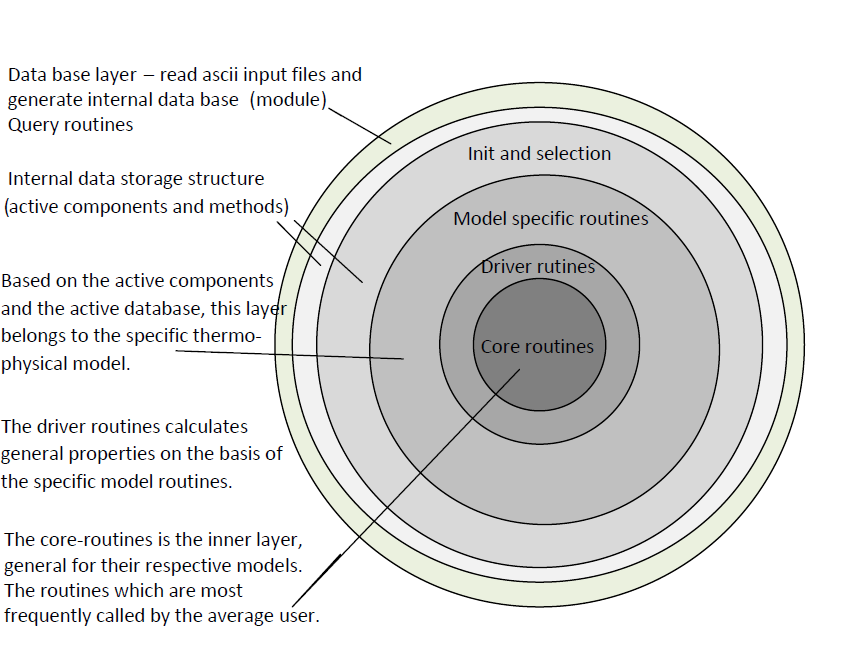
\includegraphics[width=0.70\textwidth]{eos_structure1.png}
\caption{Description of routine layers}
\label{fig:eos_structure1}
\end{figure}

The layers: \textbf{Data base layer, Internal data storage structure, initialization and
  selection structure and Driver routines} will be treated in more detail in
the next sections. Model specific routines for the general cubic equation of
state will be treated in the next sections. The following core routines will
be treated in more detail in the memo DA1202: flash calculations at specified
temperature and pressure (TP-flash), specified enthalpy and pressure
(HP-flash), specified entropy and pressure (SP-flash), specified internal
energy and volume (UV-flash) and the multiphase TP-flash.

\subsection{Input format of parameters and data}
In a thermodynamic package, each chemical component have their corresponding
data such as critical temperatures, pressures, constants for ideal gas heat
capacities and much more. The first layers in Fig. \ref{fig:eos_structure1} is
exemplified for equations of state in Fig. \ref{fig:eos_structure2}. Here it
is illustrated how parameters for the components, and also parameters for the
chosen equation of state (constants, mixing rules and interaction parameters)
are read from the database and compiled into a more condense active
structure. To make ThermoPack as flexible as possible, it has been decided to
separate the mixing rule calculations from the equation of state calculations,
such that each equation of state may be coupled to the available mixing rules
(standard, Huron-Vidal, temperature dependent, ++). To achieve a simple and
transparent program, a keyword-based data library has been chosen. An example
is shown below:

\begin{figure}[tbp]
\centering
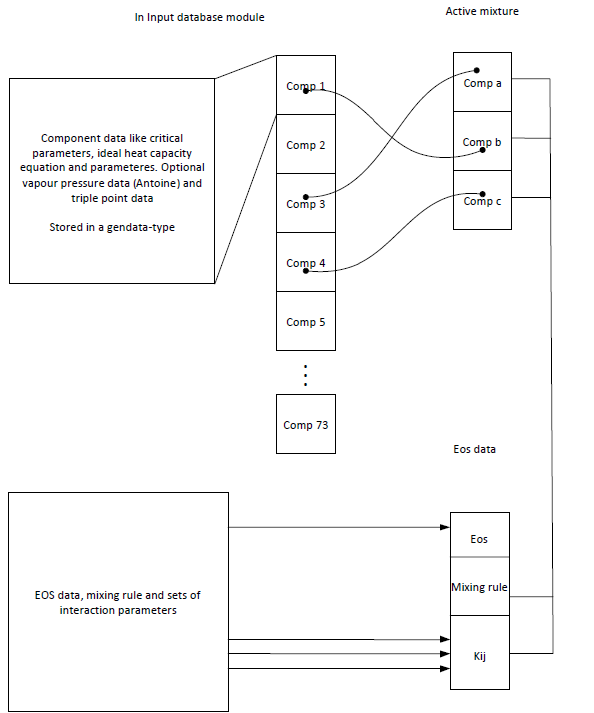
\includegraphics[width=0.70\textwidth]{eos_structure2.png}
\caption{Description of equation of state structure}
\label{fig:eos_structure2}
\end{figure}

\clearpage

\begin{verbatim}
COMP CO2
       ID = CO2
       FORMULA = CO2
       NAME = CARBONDIOXIDE_(R744)
       MW =   44.01
       TCR =   304.2
       PCR =   7376500.
       ZCR =   0.274
       ACF =   0.225
       TB =    194.7
       PSATCODE =  1
       NPSAT =  3
       ANT =   22.5898  3103.39 -0.16
       TANTMIN =   154.
       TANTMAX =   204.
       NCPTYPE =  1
       CPTYPE =  7
       NCP =  5
       CP =   0.293700E+05  0.345400E+05  0.142800E+04  0.264000E+05  0.588000E+03
       TMINCP =   50.
       TMAXCP =   5000.
 END
\end{verbatim}

Here, the currently available component data for CO$_2$ is shown. The keywords mean:

\begin{description}
\item[MW:] mole-weight [kg/kmole]
\item[TCR:] Critical temperature [K]
\item[PCR:] Critical pressure [Pa]
\item[ZCR:] Critical compressibility factor [-]
\item[ACF:] Acentric factor [-]
\item[TB:] Boiling point [K]
\item[PSATCODE:] A flag for which model which should be chosen to calculate the pure component vapour pressure
\item[NPSAT:] Number of available models for pure component vapour-pressure calculations
\item[ANT:] Antoine vapour-pressure equation coefficients 
\item[TANTMIN:] Minimum temperature for Antoine equation [K] 
\item[TANTMAX:] Maximum temperature for Antoine equation [K]
\item[NCPTYPE:] Number of available ideal gas heat capacity model
\item[CPTYPE:] Flag which refers to the ideal gas model
\item[NCP:] Number of constants in ideal gas heat capacity model
\item[CP:] Parameters in ideal gas heat capacity model
\item[TMINCP:] Minimum temperature for ideal gas heat capacity model
\item[TMAXCP:] Maximum temperature for the ideal gas heat capacity model. 
\end{description} 

New parameters can easily be included into the structure with new keywords, which makes the structure easily expanded.   

\subsection{Driver routines for equations of state}
A large number of thermodynamic state functions, derivatives and useful
relations can be obtained from all equations of state. Many of these, are
however given by the Maxwell relations, or general relations in thermodynamics
and are not specific for each equation of state. We would thus like to
implement a minimum of functions, hereby referred to as the necessary
functions, and then let other thermodynamic relations be calculated from
these. In ThermoPack, all state functions use temperature, pressure and
composition as input variables, even if these are not the canonical variables
\cite{Warberg2006}. Many choices can be made for which functions that are chosen
as necessary, but for ThermoPack, the following functions have to be supplied
for each new equation of state to be fully defined and used in most common
applications:

\begin{itemize}
\item The compressibility factor, Z
\item The enthalpy, H
\item The entropy, S
\item The fugacity coefficient, $\phi$
\end{itemize}

With these functions at hand, the other state functions may be calculated from
thermodynamic relations. Phase-equilibrium calculations at specified
temperature and pressure are available by supplying the fugacity coefficients
and compressibility factors. If the goal is to test an equation of state, and
use it in most engineering applications, numerical derivatives of the
necessary functions may be sufficiently accurate. If the thermodynamic code is
connected to fluid-dynamic calculations, or other applications which require
high accuracy for robust solution, the necessary functions must be supplied
with analytical derivatives. How this is taken care of by the driver routines
is illustrated in Fig. \ref{fig:Driver}.

\begin{figure}[tbp]
\centering
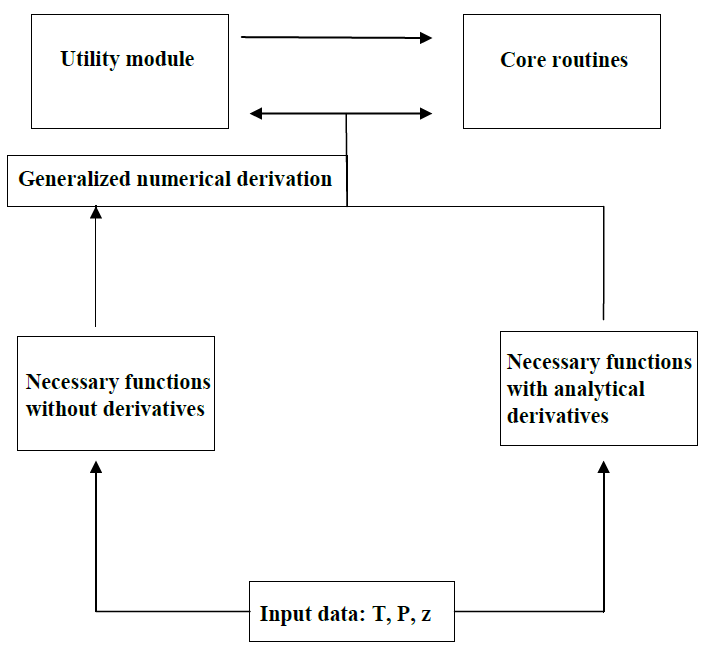
\includegraphics[width=0.70\textwidth]{driver_routines.png}
\caption{Description of the concept behind the driver routines exemplified for EoS}
\label{fig:Driver}
\end{figure}


In the functions called from the core-routines (i.e: flash-calculations,
compressibility factor solver), or the utility module (contains useful
variables and relations), the flag=1 refers to analytic derivatives, and
flag=2 refers to an automatic numerical derivation of the necessary
functions. The automatic numerical derivation methodology is expected to be
useful in the development of new CCS-thermodynamics because it means that new
EoS may be tested more efficiently.

\section{The general cubic equation of state}
\label{sec:cubicch}
Cubic Equations of State (EoS) are equations which define the pressure in a
thermodynamic system is a third-degree polynomial of the molar volume. Cubic
equations of state are probably the most used EoS in engineering calculations,
since they are simple, fast and still manage to give reasonable predictions of
densities, heat capacities and vapour-liquid equilibrium properties of
mixtures. In our computational framework, we would like to have a flexible
implementation which allows a straightforward implementation of new EoS both
to evaluate them for CCS-applications, and to equip them with suitable
interaction parameters. Table \ref{tab:eos} shows six EoS which all belong to
the cubic EoS family, but have different properties and complexity:

\begin{table}[htb]
\begin{minipage}[l]{0.58\linewidth}
\caption{Parameters used in the simulations}
\vspace{-3mm}
\begin{tabular}{| l l l |}
\hline
		&\vspace{-4mm}		&    \\
Year: 	& 	Name:	 			&         Functional form:   \\
		&\vspace{-4mm}		&    \\
\hline
		&\vspace{-4mm}		&    \\
1873	&	Van der Waals		&	$P=\frac{RT}{v-b}-\frac{a}{v^2} $ 	 \\
		&\vspace{-4mm}		&    \\

1949	&	Redlich Kwong	 	&         $P=\frac{RT}{v-b}-\frac{a/T^{0.5}}{v\left(v+b\right)}$    	 \\
		&\vspace{-4mm}		&    \\

1972	&	Soave Redlich Kwong		&	$P=\frac{RT}{v-b}-\frac{\alpha(T)a}{v\left(v+b\right)} $       	  \\
		&\vspace{-4mm}		&    \\

1976	&	Peng Robinson		&	$P=\frac{RT}{v-b}-\frac{\alpha(T)a}{v\left(v+b\right)+b(v-b)} $      	  \\

		&\vspace{-4mm}		&    \\

1980	&	Schmidt-Wensel		&	$P=\frac{RT}{v-b}-\frac{\alpha(T)a}{v^2+(1+3c)bv-3cb^2} $      \\

		&\vspace{-4mm}		&    \\

1982	&	Patel Teja			&	$P=\frac{RT}{v-b}-\frac{\alpha(T)a}{v\left(v+b\right)+c(v-b)} $        \\
		&\vspace{-4mm}		&    \\

1987	&	Yu-Lu				&	$P=\frac{RT}{v-b}-\frac{\alpha(T)a}{v\left(v+b\right)+b(3v+c)} $     \\
		&\vspace{-4mm}		&    \\

1987	&	Trebble-Bishnoi		&	$P=\frac{RT}{v-b}-\frac{\alpha(T)a}{v^2+(b(T)+c)v-b(T)c-d^2} $    \\
\hline
\end{tabular}

\label{tab:eos}
\end{minipage}
\end{table}  
  
The first four EoS; by Van der Waals, Redlich Kwong, Soave Redlich Kwong and
Peng Robinson are two-constant equations, meaning that the EoS uses only two
parameters (a and b). The three next; by Schmidt-Wensel, Patel Teja and Yu-Lu
are three parameter EoS, where the parameter "c" has been introduced. The EoS
by Trebble-Bishnoi is a four-parameter EoS with the additional parameter
"d". They can all be written in the following general expression for cubic
EoS:

\begin{equation}
P=\frac{RT}{v-b}-\frac{a\alpha(T)}{\left(v-b(T)m_1\right)\left(v-b(T)m_2\right)}
\label{eq:eosg}
\end{equation}

In all expression but the EoS by Trebble and Bishnoi, the "b"-coefficient is a
component dependent constant. This expression may be rewritten to an equation
for the compressibility factor Z:

\begin{equation}
Z=\frac{Pv}{RT}
\end{equation}

\begin{equation}
Z^3+\theta_1z^2+\theta_2z+\theta_3=0
\label{eq:theta}
\end{equation} 

Here, the parameters are:

\begin{equation}
\begin{split}
& \theta_1=-B\left(m_1+m_2\right)-B-1 \\
& \theta_2=B^2(m_1m_2)+B^2(m_1+m_2)+B(m_1+m_2)+A \\
& \theta_3= -B^3m_1m_2-B^2m_1m_2-AB \\
\end{split}
\end{equation}

Here, A is: 

\begin{equation}
A=\frac{a\alpha(T)P}{\left(RT\right)^2}
\end{equation}

and B:

\begin{equation}
B=\frac{bP}{RT}
\end{equation}

For three parameter cubic equations the C: is calculated as:
\begin{equation}
C=\frac{cP}{RT}
\end{equation}


Table 2 shows  how the constants/variables $m_1$ and $m_2$ varies with the EoS:

\begin{table}[htb]
\begin{minipage}[l]{0.58\linewidth}
\caption{$m_1$ and $m_2$ in the general cubic EoS}
\vspace{-3mm}
\begin{tabular}{| l l l |}
\hline
		&\vspace{-4mm}		&    \\
	Name:	 			&        $ m_1$ 	&	$m_2$  \\
		&\vspace{-4mm}		&    \\
\hline
		&\vspace{-4mm}		&    \\
Van der Waals:		&	0	&	0	 \\
		&\vspace{-4mm}		&    \\

Redlich Kwong:	 	&        0	&	-1   	 \\
		&\vspace{-4mm}		&    \\

Soave Redlich Kwong:		&	0	&	-1     	  \\
		&\vspace{-4mm}		&    \\

Peng Robinson:		&	-1+$\sqrt{2}$		&	-1-$\sqrt{2}$    	  \\

		&\vspace{-4mm}		&    \\

Schmidt-Wensel		&	$\frac{-1-3w+\sqrt{1+18w+9w^2}}{2}$	&	$\frac{-1-3w-\sqrt{1+18w+9w^2}}{2}$	      \\

		&\vspace{-4mm}		&    \\

Patel Teja:			&	$\frac{-b-c+\sqrt{b^2+2bc+c^2+4bc}}{2b}$	&	$\frac{-b-c-\sqrt{b^2+2bc+c^2+4bc}}{2b}$        \\
		&\vspace{-4mm}		&    \\

Yu-Lu				&	$\frac{-c-3b+\sqrt{c^2+2bc+9b^2}}{2b}$	&	$\frac{-c-3b-\sqrt{c^2+2bc+9b^2}}{2b}$	     \\
		&\vspace{-4mm}		&    \\

Trebble-Bishnoi		&	$\frac{-b(T)-c+\sqrt{b(T)^2+6b(T)c+c^2+4d}}{2b(T)}$	&  $\frac{-b(T)-c-\sqrt{b(T)^2+6b(T)c+c^2+4d}}{2b(T)}$		   \\
\hline
\end{tabular}

\label{tab:eos2}
\end{minipage}
\end{table}  

The variables $a$, $b$ $c$ are constants in all but the last EoS, where $b$ is
temperature dependent. For all but the Redlich Kwong EoS, a and b have the
following functional form:

\begin{equation}
\begin{split}
&a=\Omega_{a,i}\frac{R^2T_c^2}{P_c} \\
&b=\Omega_{b,i}\frac{RT_c}{P_c}
\end{split}
\end{equation} 



In the first four EoS in Tab. \ref{tab:eos}, $\Omega_{a,i}$ and $\Omega_{b,i}$
are constants common for all the components, the EoS by Schmidt and Wensel has
a more complicated expression for the factors, and in the EoS by Patel-Teja a
third degree polynomial in the acentric factor has to be solved for each
component at initialization. Note that for the two-parameter cubic EoS $a$ and
$b$ are chosen to satisfy the following two equations:

\begin{equation}
\left(\frac{\partial P}{\partial V}\right)_{T_c}=\left(\frac{\partial^2 P}{\partial V^2}\right)_{T_c}=0
\end{equation}


For a 3-parameter cubic equation of state the parameter $c$ is also defined:

For Patel-Teja:
\begin{equation}
c=\Omega_{c,i}\frac{RT_c}{P_c}
\end{equation} 

For Schmidt and Wenzel the acentric factor $\omega$ is used for the parameter $c$
\begin{equation}
c = \omega
\end{equation} 


Where the critical compressibility $Z_{c,i}$ is treated as a parameter that can
be fitted using the third equation:
\begin{equation}
\left(\frac{P_cV_c}{RT_c}\right) = Z_c
\end{equation}


The frequently used form by Soave for the $\alpha$-parameter is:

\begin{equation} \label{eq:alpha}
\alpha\left(T,\omega\right)=\left[1+m\left(\omega\right)\left[1-T_R^{0.5}\right]\right]^2
\end{equation}   

This expression is used also by Peng and Robinson, Schmidt and Wenzel and
Patel and Teja. To further improve the $\alpha$-parameter, the following
subject has received attention in the literature:

For the 3-parameter cubic EOS of Patel and Teja the component specific
$Z_{c,i}$ and an $m_i$ is provided in addition to the two general terms:

\begin{equation}
\begin{split}
&Z_c = 0.329032 - 0.076799\omega + 0.0211947\omega^2 \\
&m = 0.452413 + 1.30982\omega -0.295937\omega^2
\end{split}
\end{equation} 


\begin{itemize}
\item Vapour-pressures of any fluid, also polar should be well predicted.
\item The behavior of the $\alpha$-parameter in the supercritical region should be improved. 
\item Limitations at low reduced temperatures and large acentric factors should be overcome.
\end{itemize}

Many expressions have been suggested, such as the expression by Stryjek and
Vera which requires an additional parameter for each component, $k_1$ and a
function $k_0$ dependent of the component acentric factor.

\begin{equation}
\alpha\left(T,\omega\right) =\left(1+\left(k_0(\omega)+k_1(1-T_r^{0.5})/0.7-T_r)\right)(1-T_r^{0.5})\right)^2
\end{equation}



The $\alpha$-parameter should always be positive, decrease monotonically with
pressure and reach 0 at infinite temperature. The form proposed by Soave
becomes negative for some supercritical temperature and then increases. To
give a qualitatively correct $\alpha$-function, exponential functions could be
used, such as in an three parameter EoS by Yu and Lu.

Van der Waals EoS is limited to uses one constant parameter accounting for the
interaction between the components. This is the critical compressibility and
it fixed to 0.375 for all components. The EoS by Redlich Kwong gave better
description at higher pressure using the critical compressibility fixed to
0.333 for all components. 

The temperature dependence of the attractive term, $a_p$ (a product of a
temperature,acentric factor- dependent $\alpha$ and $a$), was improved by
Soave in 1972. The parameter is also correlated with the acentric factor
through the term $m$ in eq.~\ref{eq:alpha}, to include component
dependencies. Still as in Redlich Kwong, the critical compressibility is 0.333
for all components, and molar-volumes are typically overestimated. Peng
Robinson changed the expression of the second term in the pressure relation in
Eq. \ref{eq:eosg}. This improved the volume predictions, but makes PR
under-predict the saturation pressure of some fluids.

The $\alpha$-term is treated as a separate function in the core of the library
where also the analytical derivatives are developed. 

\subsection{Necessary functions for 3-parameter cubic equations of state}
A modern flexible thermodynamic library should be able to calculate important
state functions and derivatives of 3-parameter cubic equations of state, since
these are frequently used in a large variety of applications, such as in
hydrate formation predictions. In this section, it will be described how this
can be accomplished. the content in this section is a modified version of the
note by G. Owren and I.S. Melaaen from 1996 \cite{Owren1996}, adapted for
3-parameter cubic equations of state. We will restrict ourselves to mixing
rules for the parameters $b$ and $c$ that only depend on composition.


\subsection{The necessary state functions}
\label{sec:necfunc}
State functions which any decent thermodynamic package should be able to
calculate are the compressibility factor, z, the enthalpy, h, the entropy, s,
and the fugacity coefficients $\phi=f/P$. To calculate the three last, the
residual Helmholtz energy, $Y=Y_{ig}+Y_{Res}$, can be used as the starting point:

\begin{equation} \label{eq:y_TVN}
Y_{Res}(T,V,N) =\int_{V}^{\infty}\left( P -\frac{NRT}{V}\right)dV
\end{equation}

\begin{equation} \label{eq:y}
Y_{Res}(T,P,N) =\int_{V}^{\infty}\left( P -\frac{NRT}{V}\right)dV-NRT\ln(Z)
\end{equation}

A pressure function from a cubic equation of state is explicit in density and
temperature and it can often be integrated analytically. Using the reduced Helmholtz function, 
$F\equiv A/(RT)$, one obtains:
\begin{equation}
  F_{Res}(T,V,N)=\int_{V}^{\infty}\left(\frac{P}{RT}-\frac{N}{V}\right)dV=
  N\left[\ln\left(\frac{V}{V-B}\right)-\frac{A}{\left(m_1-m_2\right)BRT}\cdot\ln\left(\frac{V-m_2B}{V-m_1B}\right) \right]
\end{equation}

The residual entropy can be calculated from $F$ partial derivatives of $F$
together with the compressibility factor:

\begin{equation}
S_{Res}=\left(\frac{\partial Y_{Res}}{\partial T}\right)_{V, N_i}=(-R)\cdot \left(T\left(\frac{\partial F}{\partial T}\right)_{P,N_j}+F+N\ln(Z)\right)
\end{equation}

Moreover, the residual enthalpy is:

\begin{equation}
H_{Res}=Y_{Res}-TS_{Res}+RT\left(Z-1\right)
\end{equation}


Using ideal gas at a pressure $P$ as the reference, the fugacity coefficient is:

\begin{equation}
\ln(\phi)=\ln\left(\frac{f_i}{P}\right)=\frac{\mu_{i,Res}}{RT}=\frac{1}{RT}\left(\frac{\partial Y_{Res}}{\partial N_i}\right)_{T,P,N_j}=\left(\frac{\partial F}{\partial N_i}\right)_{T,P,N_j}-\ln(Z)
\end{equation}

The necessary functions to do flash-calculations with numerical derivatives
are given above, combined with ($\partial F/\partial T$)$_{P,N,i}$ for entropy
an ($\partial F/\partial N_i$)$_{T,P}$ for the fugacities.  Since a pressure
function is the most common way to represent cubic equations of state, and the
F-function plays an important role in the necessary state function, analytical
derivatives will be given below, first for the reduced Helmholtz-function and then for the 
pressure

\subsection{The reduced Helmholtz-function - simplified}

The reduced residual Helmholtz free energy function, $F$, for a general cubic
equation of state with two or three parameters (A,B and C) can be expressed as

\begin{equation}
  \label{eq:1}
  F = F(N,T,V,D,B,C) = -Ng(V,B) - \frac{A(T)}{T} f(V,B,C)
\end{equation}
where $g$ is defined as: 
\begin{equation}
  \label{eq:2}
  g = \ln(1-\frac{B}{V}) = \ln(V-B) - \ln V
\end{equation}
and  $f$ is defined as:
\begin{equation}
  \label{eq:3}
  f = \frac{1}{R \cdot B\left(m_1 - m_2\right)}\ln \frac{V-m_2 B}{V-m_1 B}
\end{equation}

in the $f$-function the $m_1$ and $m_2$ can both be functions of $B$ and the
third parameter $C$. In some cases $B$ and $C$ can be functions of temperature
also.

In the implementation, the following short-functions are used:
\begin{eqnarray}
  n_1 (V,B,C) & = & V - m_1B \\
  n_2 (V,B,C) & = & V - m_2B \\
  n(V,B)      & = & V - B \\
  m(B,C)      & = & m_1 - m_2 \\\
  h(V,B,C)    & = & \ln{\left(\frac{n_2}{n_1}\right)} = \ln{n_2}-\ln{n_1}
\end{eqnarray}

Then the $f$ and $g$-function can be expressed as:
\begin{eqnarray}
  \label{eq:4}
  f &= &\frac{h}{m \cdot R \cdot B} \\
  g &= &\ln n - \ln V
\end{eqnarray}

The total number of moles $N$ is:
\begin{equation}
  \label{eq:5}
  N = \sum_i N_i
\end{equation}

The temperature dependent parameter $A$ is defined as $N^2 a_{mix}$, $B=\sum_i
N_i b_{ii}$ and $C = \sum_i c_{ii}$. 

The mixing rules are discussed further in section~\ref{sec:mixing}


\subsubsection{Partial derivatives of  $F$ for calculation of thermodynamic properties}

The partial derivatives required for the various thermodynamic properties are
listed next.

For making the derived it is asumed A and B is a function of composition and temperaturee where C is only a function of composition. This can be written:
\begin{equation}
F=F\left(N,T,A(N,T),B(N,T),C(N)\right)
\end{equation}

\textbf{First order derivatives}

\noindent\hrulefill

\begin{equation}
\left(\frac{\partial F}{\partial N_i}\right)_{T,V,Nj}=F_N+F_A\cdot A_i+F_B\cdot B_i+F_{C}\cdot C_i 
\end{equation}

\noindent\hrulefill

\begin{equation}
\left(\frac{\partial F}{\partial T}\right)_{V,{\mathbf{N}}}=F_{T}+F_{A}\cdot A_{T}+F_{B}\cdot B_{T}
\end{equation} 

\noindent\hrulefill

\begin{equation}
\left(\frac{\partial F}{\partial V}\right)_{T,{\mathbf N}} = F_V
\end{equation}


\noindent\hrulefill\\

\textbf{Second order derivatives}

 The development of the second order derived is not straight forward and the development of the formula is of that reason shown: 

\noindent\hrulefill

\begin{equation}
\begin{split}
\left(\frac{\partial^2 F}{\partial T\partial N_{i}}\right)_{V,N_{j}}=\frac{\partial}{\partial T}\left(\frac{\partial F}{\partial N_{i}}\right)=\frac{\partial}{\partial T}\left(F_{N}+F_{A}A_{i}+F_{B}B_{i}+F_{C}C_{i}\right)\\
\mbox{}=\frac{\partial F_{n}}{\partial T}+F_{A}\frac{\partial A_{i}}{\partial T}+A_{i}\frac{\partial F_{A}}{\partial T}+F_{B}\frac{\partial B_{i}}{\partial T}+B_{i}\frac{\partial F_{B}}{\partial T}+C_{i}\frac{\partial F_{C}}{\partial T}\\
=F_{NT}+F_{NA}A_{T}+F_{NB}B_{T}\\
+F_{A}A_{iT}+A_{i}\left(F_{AT}+F_{AA}A_{T}+F_{AB}B_{T}\right)\\
+F_{B}B_{iT}+B_{i}\left(F_{BT}+F_{BA}A_{T}+F_{BB}B_{T}\right)\\
+C_{i}\left(F_{CT}+F_{CA}A_{T}+F_{CB}B_{T}\right)
\end{split}
\end{equation} 

\noindent\hrulefill

\begin{equation}
\begin{split}
\left(\frac{\partial^2 F}{\partial N_{j}\partial N_{i}}\right)_{T,V}=\frac{\partial}{\partial N_{j}}\left(\frac{\partial F}{\partial N_{i}}\right)=\frac{\partial}{\partial N_{j}}\left(F_{N}+F_{A}A_{i}+F_{B}B_{i}+F_{C}C_{i}\right)\\
\mbox{}=\frac{\partial F_{n}}{\partial N_{j}}+F_{A}\frac{\partial A_{i}}{\partial N_{j}}+A_{i}\frac{\partial F_{A}}{\partial N_{j}}+F_{B}\frac{\partial B_{i}}{\partial N_{j}}+B_{i}\frac{\partial F_{B}}{\partial N_{j}}+C_{i}\frac{\partial F_{C}}{\partial N_{j}}\\
=F_{NN}+F_{NA}A_{j}+F_{NB}B_{j}+F_{NC}C_{j}\\
+F_{A}A_{ij}+A_{i}\left(F_{AN}+F_{AA}A_{j}+F_{AB}B_{j}+F_{AC}C_{j}\right)\\
+F_{B}B_{ij}+B_{i}\left(F_{BN}+F_{BA}A_{j}+F_{BB}B_{j}+F_{BC}C_{j}\right)\\
+F_{C}C_{ij}+C_{i}\left(F_{CN}+F_{CA}A_{j}+F_{CB}B_{j}+F_{CC}C_{j}\right)
\end{split}
\end{equation} 
It is her used that $F_{NN}=F_{NA}=F_{NC}=0$ and that therm is then
not incldued in the code

\noindent\hrulefill

\begin{equation}
\begin{split}
\left(\frac{\partial^2 F}{\partial T^2}\right)_{V,N}=\frac{\partial}{\partial T}\left(\frac{\partial F}{\partial T}\right)=\frac{\partial}{\partial T}\left(F_{T}+F_{A}A_{T}+F_{B}B_{T}\right)\\
\mbox{}=\frac{\partial F_{T}}{\partial T}+F_{A}\frac{\partial A_{T}}{\partial T}+A_{T}\frac{\partial F_{A}}{\partial T}+F_{B}\frac{\partial B_{T}}{\partial T}+B_{T}\frac{\partial F_{B}}{\partial T}\\
=F_{TT}+F_{TA}A_{T}+F_{TB}B_{T}\\
+F_{A}A_{TT}+A_{T}\left(F_{AT}+F_{AA}A_{T}+F_{BA}B_{T}\right)\\
+F_{B}B_{TT}+B_{T}\left(F_{BT}+F_{BA}A_{T}+F_{BB}B_{T}\right)\\
=F_{TT}+2F_{TA}A_{T}+2F_{TB}B_{T}\\
+F_{A}A_{TT}+F_{B}B_{TT}\\
+F_{AA}A_{T}^{2}+2F_{AB}A_{T}B_{T}+F_{BB}B_{T}^{2}
\end{split}
\end{equation} 

\noindent\hrulefill

The partial derivatives of the $F$-function is listed next.

\subsubsection{The partial derivatives of $F$-function}

\textbf{First order derivatives}\\

\noindent\hrulefill

\begin{equation}
F_N = -g
\end{equation}

\noindent\hrulefill

\begin{equation}
F_A= -\frac{f}{T}
\end{equation}

\noindent\hrulefill

\begin{equation}
F_B = -g_B - \frac{A}{T}f_B
\end{equation}

\noindent\hrulefill

\begin{equation}
F_C = -\frac{A}{T} f_C
\end{equation}

\noindent\hrulefill

\begin{equation}
  F_T = \frac{A}{T^2} f
\end{equation}

\noindent\hrulefill

\begin{equation}
  F_{AB} = -\frac{f_B}{T}
\end{equation}

\noindent\hrulefill

\begin{equation}
  F_{AC} = -\frac{f_C}{T}
\end{equation}

\noindent\hrulefill

\begin{equation}
  F_{AT} = \frac{f}{T^2}
\end{equation}

\noindent\hrulefill

\begin{equation}
  F_{BB} = -g_{BB} - \frac{A}{T} f_{BB}
\end{equation}

\noindent\hrulefill

\begin{equation}
  F_{BC} = -\frac{A}{T} f_{BC}
\end{equation}

\noindent\hrulefill

\begin{equation}
  F_{BT} = \frac{A}{T^2} f_{B}
\end{equation}

\noindent\hrulefill

\begin{equation}
  F_{CT} = \frac{A}{T^2} f_{C}
\end{equation}

\noindent\hrulefill

\begin{equation}
  F_{CC} = -\frac{A}{T} f_{CC}
\end{equation}

\noindent\hrulefill

\begin{equation}
  F_{TT} = -2.0 \frac{F_T}{T}
\end{equation}

\noindent\hrulefill

\begin{equation}
  F_{V} = -g_V - \frac{A}{T} f_V
\end{equation}

\noindent\hrulefill

\begin{equation}
  F_{NV} = -g_V
\end{equation}

\noindent\hrulefill

\begin{equation}
  F_{NB} = -g_B
\end{equation}

\noindent\hrulefill

\begin{equation}
  F_{VT} = \frac{A}{T^2} f_V
\end{equation}

\noindent\hrulefill

\begin{equation}
  F_{VV} = -g_{VV} - \frac{A}{T} f_{VV}
\end{equation}

\noindent\hrulefill

\begin{equation}
  F_{VA} = -\frac{f_{V}}{T}
\end{equation}

\noindent\hrulefill

\begin{equation}
  F_{VB} = -g_{VB} - \frac{A}{T} f_{VB}
\end{equation}

\noindent\hrulefill

\begin{equation}
  F_{VC} = -\frac{A}{T} f_{VC}
\end{equation}

\noindent\hrulefill

The following derivatives are zero: $F_{NN}$, $F_{NT}$, $F_{NA}$,
$F_{AA}$ and $F_{NC}$

\subsubsection{Derivatives of the helper functions $f$ and $g$}

With the help of the notations described above:

\begin{equation}
  f_{V} = \frac{h_V}{m \cdot B \cdot R}
\end{equation}

\noindent\hrulefill

\begin{equation}
%  f_{B} = \frac{1}{m \cdot B \cdot R}\left(h_B - \frac{h}{m} m_B - \frac{h}{B}\right)
  f_B = \frac{h_B}{m\cdot B \cdot R} - \frac{f}{B} - \frac{f\cdot m_B}{m}
\end{equation}

\noindent\hrulefill

\begin{equation}
%  f_{C} = \frac{1}{m \cdot B \cdot R}\left(h_C - \frac{h}{m} m_C \right)
  f_C = \frac{h_C}{m\cdot B \cdot R} - \frac{f\cdot m_C}{m}
\end{equation}

\noindent\hrulefill

\begin{equation}
  f_{VV} = \frac{h_{VV}}{ m \cdot B \cdot R}
\end{equation}

\noindent\hrulefill

\begin{equation}
  f_{VB} = \frac{1}{m \cdot B \cdot R} \left(h_{VB} - \frac{h_V}{m}m_B - \frac{h_V}{B}\right)
\end{equation}

\noindent\hrulefill

\begin{equation}
  f_{VC} = \frac{1}{m \cdot B \cdot R} \left(h_{VC} - \frac{h_V}{m}m_C \right)
\end{equation}

\noindent\hrulefill

\begin{equation}
%\begin{split}
 f_{BB} = \frac{1}{m\cdot B \cdot R}\left[h_{BB} - R\left(2 f_B\left(m+m_B\right) +f\left(m_B+m_{BB}\right)\right)\right]
%  f_{BB} = \frac{1}{m \cdot B \cdot R}\left(h_{BB} - \frac{2 h_B m_B + h m_{BB}}{m}
% - \frac{2 h_B}{B} + \frac{2 h m_B^2}{m^2} + \frac{2 h m_B}{m B}\right)
%\end{split}
\end{equation}

\noindent\hrulefill

\begin{equation}
%  \begin{split}
  f_{BC} = \frac{1}{m \cdot B \cdot R} \left(h_{BC} - \frac{h_B m_C + h_C m_B + h m_{BC}}{m}
+ \frac{2 h m_B m_C}{m^2} - \frac{h_C}{B^2}\right)
%\end{split}
\end{equation}

\noindent\hrulefill

\begin{equation}
%\begin{split}
  f_{CC} = \frac{1}{m \cdot B \cdot R} \left(h_{CC} - \frac{2 h_C m_C + h m_{CC}}{m} 
 + \frac{2 h m_C^2}{m^2}\right)
%\end{split}
\end{equation}

\noindent\hrulefill

\begin{equation}
  g_{V} = \frac{1}{n} - \frac{1}{V} 
\end{equation}

\noindent\hrulefill

\begin{equation}
  g_{B} = -\frac{1}{n}
\end{equation}

\noindent\hrulefill

\begin{equation}
  g_{VV} = -\frac{1}{n^2} + \frac{1}{V^2}
\end{equation}

\noindent\hrulefill

\begin{equation}
  g_{VB} = \frac{1}{n^2} 
\end{equation}

\noindent\hrulefill

\begin{equation}
  g_{BB} = -g_{VB}
\end{equation}

The partial derivatives of $h$, $m$, $n_1$, $n_2$ and $n$ are listed in the
appendix for completeness.

\noindent\hrulefill


\newpage

\subsection{The pressure function with derivatives}

The pressure and the derivatives are often needed and although the pressure
with the derivatives are directly described from the $F$-function in the
previous section, it is convenient to have these directly available.

With the mixing parameters scaled to: $A=N^2a\alpha(T)$ and $B=Nb$. the equation in \ref{eq:eosg} may be rewritten as:

From the $F$-function the pressure is expressed as:
\begin{equation}
  \label{eq:6}
  P = R \cdot T\left( -F_V + \frac{1}{V}\right)    
\end{equation}

 or 
\begin{equation}
  P=\frac{NRT}{V-B}+\frac{A}{\left(V-Bm_1\right)\left(V-Bm_2\right)} 
\label{eq:eosg2}
\end{equation}

With the short-functions used in the implementation 
\begin{equation}
  \label{eq:7}
  p = \frac{R \cdot T}{n} - \frac{A}{n_1 \cdot n_2}
\end{equation}
where (repeated):
\begin{eqnarray*}
  n &=& V-B \\
  n1 &=& V-m_1B \\
  n2 &=& V-m_2B
\end{eqnarray*}


\subsubsection{The derivatives of P($N$,$V$,$T$,$A$,$B$,$C$)}

With $a_p=a\alpha(T)$, the derivatives of the pressure with respect to the
total number of moles, $N$, the volume $V$, the temperature, $T$, and the
parameters $A$, $B$ and $C$  are:

\noindent\hrulefill

\begin{equation}
N \cdot P_N=N\cdot\frac{\partial P}{\partial N}=\frac{R\cdot T}{V-B}
\end{equation}

\noindent\hrulefill

\begin{equation}
N\cdot P_V=\frac{-RT}{(V-B)^2}+a_p\frac{n_1+n_2}{\left(n_1\cdot n_2\right)^2}
\end{equation}

\noindent\hrulefill

\begin{equation}
N^2P_A=N^2\cdot\frac{\partial P}{\partial A}=\frac{-1}{n_1\cdot n_2}
\end{equation}

\noindent\hrulefill

\begin{equation}
N\cdot P_B=N\cdot \frac{\partial P}{\partial B}=\frac{RT}{\left(V-B\right)^2}-a_p\cdot\frac{\left(m_1 + B\cdot m_{1,B}\right)\cdot n_2 
   +\left(m_2 + B \cdot m_{2,B} \right) \cdot n_2}{\left(n_1\cdot n_2\right)^2}
\end{equation}

\noindent\hrulefill

\begin{equation}
N\cdot P_C=N\cdot \frac{\partial P}{\partial C}= -R \cdot A \cdot F_{VC}
\end{equation}

\noindent\hrulefill

\begin{equation}
P_T=\frac{\partial P}{\partial T}=\frac{T}{V-B}
\end{equation}

\noindent\hrulefill

\subsubsection{The derivatives of P($T$,$V$,$N_i$)}
Assuming that $m_1$ and $m_2$ are both functions of $B$ and an additional
parameter $C$, the pressure derivatives are:

\noindent\hrulefill

\begin{equation}
\left(\frac{\partial P}{\partial N_i}\right)_{T,V,N_j}=P_N+P_A\cdot A_i+P_B\cdot B_i + P_{C}\cdot C_i
\end{equation}

\noindent\hrulefill

\begin{equation}
\left(\frac{\partial P}{\partial V}\right)_{T,{\mathbf N}} = P_V
\end{equation}

\noindent\hrulefill

\begin{equation}
\left(\frac{\partial P}{\partial T}\right)_{V,{\mathbf N}} = P_T+P_A\cdot A_T+P_B\cdot B_T + P_C \cdot C_T
\end{equation}

Without temperature dependency in $B$ and $C$ the terms $B_T$ and $C_T$ becomes zero.

\noindent\hrulefill



\newpage
\subsection{Mixing rules}
With the expression for the pressure and f-function derivatives at hand, we
have still not defined the composition derivatives of the mixing rules which
will dictate the composition dependency of the $m_1$ and $m_2$
parameters. This section contains these derivatives for both the standard and
the Huron-Vidal mixing rules, and also the composition derivatives of, $m_1$
and $m_2$ for the 3-parameter cubic EoS by Schmidt and Wensel described
previously.

\subsubsection{Standard mixing rules}
\label{sec:mixing}

For the parameters $a_p$ and $B$, the mixing rules are:

\begin{equation}
B=\sum_ix_ib_i
\end{equation}

\begin{equation}
A=\sum_i\sum_jx_ix_ja_{p,ij}
\end{equation}

\begin{equation}
a_{p,ij}=\sqrt{a_{p,i}a_{p,j}}\left(1-k_{ij}\right)
\end{equation}

If we make the a and b not composition dependent, $A=N^2a$ and $B=Nb$ this
results in the following composition derivatives:

\noindent\hrulefill

\begin{equation}
\frac{1}{N}A_i=\frac{1}{N}\frac{\partial A}{\partial N_i}=2\sum_jx_ja_{p,ij}
\end{equation}

\noindent\hrulefill

\begin{equation}
\frac{1}{N}A_{iT}=\frac{1}{N}\frac{\partial^2 A}{\partial N_i \partial T}=2\sum_jx_j\frac{d a_{p,ij}}{dT}
\end{equation}

\noindent\hrulefill

\begin{equation}
\frac{1}{N^2}A_{T}=\frac{1}{N^2}\frac{\partial A}{\partial T}=\frac{1}{2}\sum_ix_i\frac{A_{iT}}{N}
\end{equation}

\noindent\hrulefill

\begin{equation}
\frac{1}{N^2}A_{TT}=\frac{1}{N^2}\frac{\partial^2 A}{\partial T^2}=\sum_i x_i \sum_j x_j\frac{\partial^2 a_{p,ij}}{\partial T^2}
\end{equation}

\noindent\hrulefill

\begin{equation}
B_{i}=\frac{\partial B}{\partial N_i}=b_i
\end{equation}

\noindent\hrulefill

\begin{equation}
\frac{da_{p,ij}}{dT}=\left(1-k_{ij}\right)\cdot\frac{1}{2\sqrt{a_{p,i}a_{p,j}}}\cdot\left(a_{p,i}\frac{da_{p,j}}{dT}+a_{p,j}\frac{da_{p,i}}{dT}\right)
\end{equation}

\noindent\hrulefill

\begin{equation}
\frac{d^2a_{p,ij}}{dT^2}=\frac{1-k_{ij}}{2}\cdot\left(\frac{2\frac{da_{p,i}}{dT}\frac{da_{p,j}}{dT}+a_{p,i}\frac{d^2a_{p,j}}{dT^2}+a_{p,j}\frac{d^2a_{p,i}}{dT^2}}{\sqrt{a_{p,i}a_{p,j}}}-\frac{\left(a_{p,i}\frac{da_{p,j}}{dT}+a_{p,j}\frac{da_{p,i}}{dT}\right)^2}{2\sqrt{a_{p,i}a_{p,j}}a_{p,i}a_{p,j}}\right)
\end{equation}


\noindent\hrulefill

\textbf{The derivatives of the $m_1$ and $m_2$ functions}\\

For Schmidt and Wensel:

\begin{equation}
\left(\frac{\partial m_1}{\partial C}\right)=-\frac{3}{2}+\frac{9+9C}{2\sqrt{1+18C+9C^2}}
\end{equation}

\begin{equation}
\left(\frac{\partial m_2}{\partial C}\right)=-\frac{3}{2}-\frac{9+9C}{2\sqrt{1+18C+9C^2}}
\end{equation}

\begin{equation}
\left(\frac{\partial^2m_1}{\partial C^2}\right)=\frac{9}{2\sqrt{1+18C+9C^2}}-\frac{9+9C}{4\left(1+18C+9C^2\right)^{1.5}}
\end{equation}

\begin{equation}
\left(\frac{\partial^2m_2}{\partial C^2}\right)=-\left(\frac{\partial^2 m_1}{\partial C^2}\right)
\end{equation}


For Patel-Teja Equation of state:

% \begin{equation}
%  \frac{d m_1}{d N_i}= \frac{d m_1}{d B}\frac{\partial B}{\partial N_{i}} +\frac{d m_1}{d C}\frac{\partial C}{\partial N_{i}} 
% \end{equation}

% \begin{equation}
% M_{2,i}=\frac{d m_2}{d N_i}=\frac{d m_2}{d B}\frac{\partial B}{\partial N_{i}} +\frac{d m_2}{d C}\frac{\partial C}{\partial N_{i}} 
% \end{equation}

% \begin{equation}
% M_{1,ij}=\frac{\partial^2 m_1}{\partial N_i \partial N_j}=\frac{d^2 m_1}{dB^2} b_i b_j +\frac{d^2 m_1}{d C^2} c_i c_j
% \end{equation}

% \begin{equation}
% M_{2,ij}=\frac{\partial^2 m_2}{\partial N_i \partial N_j}=\frac{d^2 m_2}{dB^2} b_i b_j +\frac{d^2 m_2}{d C^2} c_i c_j
% \end{equation}

With $m_1$ and $m_2$ defined as:
\begin{eqnarray}
  \label{eq:9}
  m_1 &=& \frac{-B - C + \sqrt{D}}{2 B}\\
  m_2 &=& \frac{-B - C - \sqrt{D}}{2 B}
\end{eqnarray}

With:  $D = B^2 + 6\cdot B\cdot C + C^2$

The derivatives are the following:

\begin{eqnarray}
  \left(\frac {\partial m_1}{\partial B}\right) &=& -\frac{C\cdot\left(3\cdot B - \sqrt{D} + C\right)}{2\sqrt{D}B^2} \\
  \left(\frac {\partial m_2}{\partial B}\right) &=& \frac{C\cdot\left(3\cdot B + \sqrt{D} + C\right)}{2\sqrt{D}B^2} \\
  \left(\frac {\partial m_1}{\partial C}\right) &=& \frac{3\cdot B + C - \sqrt{D}} {2\sqrt{D} B} \\
  \left(\frac {\partial m_2}{\partial C}\right) &=& -\frac{3\cdot B + C + \sqrt{D}} {2\sqrt{D} B}
\end{eqnarray}

\noindent\hrulefill\\

The second order derivatives of $B$ and $C$

With the help of the following definitions:

\begin{eqnarray}
  \label{eq:14}
  D & = & B^2 + 6\cdot B\cdot C + C^2 \\  
  F & = & 3B + C \\
  G & = & B^2 + 5 \cdot B \cdot C + 3 C^2 \\
  H & = & B^3\cdot D \cdot \sqrt{D}
\end{eqnarray}
  
the second order derivatives are:

\begin{equation}
  \label{eq:15}
  \left(\frac{\partial^2 m_1}{\partial B^2}\right) = 
  \frac{C\left(3B \cdot G - D\sqrt{D} + C^3\right)}{H}
\end{equation}

\begin{equation}
  \label{eq:16}
  \left(\frac{\partial^2 m_2}{\partial B^2}\right) = 
  -\frac{C\left(3B\cdot G + D\sqrt{D} + C^3\right)}{H}
\end{equation}

\begin{equation}
  \label{eq:17}
  \left(\frac{\partial^2 m_1}{\partial C^2}\right) = 
  -\frac{F^2 - D}{2 B \cdot D\sqrt{D}}
\end{equation}

\begin{equation}
  \label{eq:18}
  \left(\frac{\partial^2 m_2}{\partial C^2}\right) = 
  -\left(\frac{\partial^2 m_1}{\partial C^2}\right)
\end{equation}

The cross derivatives are:

\begin{equation}
  \label{eq:19}
  \left(\frac{\partial^2 m_1}{\partial B \partial C}\right) = 
  -\frac{\left(E-\sqrt{D}\right) \cdot \left(B\left(B+3C\right)-C\sqrt{D}\right)}{2 D\sqrt{D}B^2}
\end{equation}

\begin{equation}
  \label{eq:20}
  \left(\frac{\partial^2 m_2}{\partial B \partial C}\right) = 
  \frac{\left(E+\sqrt{D}\right) \cdot \left(B\left(B+3C\right)+C\sqrt{D}\right)}{2 D\sqrt{D}B^2}
\end{equation}

\noindent\hrulefill\\



\subsubsection{Mixing rule for $B$ and $C$ in the 3-parameter cubic EOS}


The standard mixing rules for in Schmidt and Wensel:

\begin{equation}
C=\frac{\sum_rx_rw_rb_r^{0.7}}{\sum_kx_kb_k^{0.7}}
\end{equation}

Introducing the two variables $\gamma_1$ and $\gamma_2$ as:

\begin{eqnarray}
  \label{eq:8}
  \gamma_1 &=& \sum_rx_rw_rb_r^{0.7} \\
  \gamma_2 &=& \sum_kx_kb_k^{0.7}
\end{eqnarray}

Gives the following derivatives:

\begin{equation}
N\cdot C_i=N\cdot\frac{d c}{d N_i}=\frac{b_i^{0.7}}{\gamma_2} \left(w_i - \frac{\gamma_1}{\gamma_2}\right)
\end{equation}

and

\begin{equation}
N^2\cdot C_{ij}=N^2\cdot\left(\frac{\partial^2 C}{\partial N_iN_j}\right)=
   -\frac{b_i^{0.7}b_j^{0.7}}{\gamma_2^2}\left(w_i+w_j-2\frac{\gamma_1}{\gamma_2}\right)
\end{equation}

\noindent\hrulefill

The standard mixing rule for Patel Teja:

\begin{equation}
  C=N\cdot\sum_ix_ic_i
\end{equation}
and 
\begin{equation}
  B=N\cdot\sum_ix_ib_i
\end{equation}

Gives the following derivatives:

\begin{equation}
N\cdot C_i=N\cdot\left(\frac{\partial C}{\partial N_i}\right)=c_i
\end{equation}
and
\begin{equation}
N\cdot B_i=N\cdot\left(\frac{\partial B}{\partial N_i}\right)=b_i
\end{equation}

\noindent\hrulefill

The second derivatives $B_{ij}$ and $C_{ij}$ are zero.


\subsubsection{The Huron Vidal mixing rule}
To have the Huron-Vidal mixing rule as a equivalent mixing rule as the
standard mixing rule by van der Waals in our thermodynamic package, analytical
derivatives have to be supplied. The Huron-Vidal mixing rule is for the
mixture parameter a:

\begin{equation}
a=b\left[\sum_{z=1}^N\left(x_z\frac{a_z}{b_z}\right)-\frac{G_{\infty}^E}{\ln{2}}\right]
\end{equation}

(Note: The $a_z$-parameter is here the $a_p$ parameter described earlier as  $\alpha(T) a$)
Here, the excess Gibbs energy at infinite pressure is:

\begin{equation}
G_{\infty}^E=RT\sum_{z=1}^Nx_z\frac{\sum_{r=1}^N\tau_{rz}b_rx_rC_{rz}}{\sum_{k=1}^N b_kx_kC_{kz}}
\end{equation}

Moreover, the other parameters are:

\begin{equation}
\tau_{rz}=\frac{\Delta g_{rz}}{RT}
\end{equation}

\begin{equation}
C_{rz}=\exp{(-\alpha_{rz}\tau_{rz})}
\end{equation}

Here, $\alpha_{ji}$ are typically constants, while $\Delta g_{ji}$ are either first degree polynomials in the temperature (HV1):

\begin{equation}
\tau_{rz}=\frac{1}{R}\left(\frac{a_{rz}}{T}+b_{rz}\right)
\end{equation}

or second degree polynomials (HV2):

\begin{equation}
\tau_{rz}=\frac{1}{R}\left(\frac{a_{rz}}{T}+b_{rz}+c_{rz}T\right)
\end{equation}

For interactions between non-polar components were specific values for
$\alpha$ and $\tau$ has not been fitted, the mixing-rule falls back to the standard Van der Waals
mixing rule with one interaction parameter $k_{ij}$ if the excess energy
parameters are chosen as:

\begin{eqnarray}
\alpha_{ij} & = & 0\\
g_{ii} & = & \frac{a_{i}}{b_{i}}\Delta\\
g_{ji} & = & -2\frac{\sqrt{b_i b_j}}{b_i + b_j}\sqrt{g_{ii}g_{jj}}\left(1-k_{ij}\right)\\
\tau_{ji} &=& \frac{g_{ji}-g_{ii}}{RT} 
\end{eqnarray}


($\Delta$ = $\ln{2}$ for SRK, 1.0 for VdW and 0.623 for the PR EOS)

The 1st and 2nd derivative of the $\tau$-function are also developed.  Using
the above equations with the Huron-Vidal mixing rule, is fully consistent and
equivalent to using SRK with VdW mixing rule. This is very convenient to use
for a mixture containing polar and non-polar substances avoiding too much
``bookkeeping'' in the implementation.

\noindent\hrulefill


\textbf{The temperature derivative, $\frac{dA}{dT}$ (checked numerically)}\\
The overall expression:

\begin{equation}
\frac{1}{N^2}\frac{\partial A}{\partial T}=b\left[\sum_{z=1}^N\left(x_z\frac{1}{b_z}\right)\frac{\partial a_z}{\partial T}-\frac{1}{\ln{2}}\frac{\partial G_{\infty}^E}{\partial T}\right]
\end{equation}

and then:

\begin{equation}
\begin{split}
&\frac{\partial G_{\infty}^E}{\partial T}=R\sum_{z=1}^N x_z\frac{\sum_{r=1}^N\tau_{rz}b_rx_rC_{rz}}{\sum_{k=1}^n b_kx_kC_{kz}}+\\
&RT\sum_{z=1}^N x_z\left(\frac{\sum_{r=1}^N\tau_{rz}b_rx_rC_{rz}}{\left(\sum_{k=1}^N b_kx_kC_{kz}\right)^2}\sum_{k=1}^N b_kx_k\alpha_{kz}C_{kz}\frac{\partial \tau_{kz}}{\partial T}\right)+ \\
&RT\sum_{z=1}^N x_z\left(\frac{\sum_{r=1}^N \frac{\partial \tau_{rz}}{\partial T}b_rx_rC_{rz}-\alpha_{rz}\tau_{rz}\frac{\partial \tau_{rz}}{\partial T}b_rx_rC_{rz}}{\sum_{k=1}^N b_kx_kC_{kz}}\right)
\end{split}
\end{equation}

The first and second temperature derivatives of $\tau$ (HV1):

\begin{equation}
\frac{\partial \tau_{rz}}{\partial T}=\frac{1}{R}\left(-\frac{a_{rz}}{T^2}\right)\hspace{2cm}\frac{\partial^2 \tau_{rz}}{\partial T^2}=\frac{1}{R}\left(\frac{2a_{rz}}{T^3}\right)
\end{equation}

The first and second temperature derivatives of $\tau$ (HV2):

\begin{equation}
\frac{\partial \tau_{rz}}{\partial T}=\frac{1}{R}\left(-\frac{a_{rz}}{T^2}+c_{rz}\right)\hspace{2cm}\frac{\partial^2 \tau_{rz}}{\partial T^2}=\frac{1}{R}\left(\frac{2a_{rz}}{T^3}\right)
\end{equation}

\noindent\hrulefill\\

\textbf{The composition derivative, $\frac{dA}{dN_i}$ (checked numerically)}\\
The overall expression:

\begin{equation}
\frac{1}{N}\frac{\partial A}{\partial N_i}=b_i\cdot \left[\sum_{z=1}^N\left(x_z\frac{a_z}{b_z}\right)-\frac{G_{\infty}^E}{\ln{2}}\right]+b\left[\frac{a_i}{b_i}-\frac{1}{\ln{2}}\cdot\frac{\partial \left(G_{\infty}^E\cdot N\right)}{\partial N_i}\right]
\end{equation}

where:

\begin{equation}
\frac{\partial \left(G_{\infty}^E\cdot N\right)}{\partial N_i}=RT\cdot\left(\frac{\sum_{r=1}^N\tau_{ri}b_rx_rC_{ri}}{\sum_{k=1}^N b_kx_kC_{ki}}
+\sum_{z=1}^N\frac{x_z\tau_{iz}b_iC_{iz}}{\sum_{k=1}^N b_kx_kC_{kz}}- \sum_{z=1}^N x_zb_iC_{iz}\frac{\sum_{r=1}^N\tau_{rz}b_rx_rC_{rz}}{\left(\sum_{k=1}^N b_kx_kC_{kz}\right)^2}\right) 
\end{equation}

\noindent\hrulefill\\

\textbf{The second degree composition derivative, $\frac{d^2A}{dN_idN_j}$}\\
The overall expression:

\begin{equation}
  \frac{\partial^2 A}{\partial N_i \partial N_j}=b_i\cdot \left[\frac{a_j}{b_j}-\frac{1}{\ln{2}}\frac{\left(G_{\infty}^E\cdot N\right)}{\partial N_j}\right]
  +b_j\left[ \frac{a_i}{b_i}-\frac{1}{\ln{2}}\cdot\frac{\partial \left( G_{\infty}^E\cdot N\right)}{\partial N_i}\right]-\frac{b\cdot N}{\ln{2}}\cdot \frac{\left(\partial G_{\infty}^E\cdot N\right)}{\partial N_i \partial N_j}
\end{equation}

% +b_j\left[ \frac{a_i}{b_i}-\frac{1}{\ln{2}}\cdot\frac{\partial \left(
%     G_{\infty}^E\cdot N\right)}{\partial N_i}\right]+\frac{b\cdot
% N}{\ln{2}}\cdot \frac{\left(\partial G_{\infty}^E\cdot N\right)}{\partial
% N_i \partial N_j}

where:

\begin{equation}
\begin{split}
&\frac{\partial^2 \left(G_{\infty}^E\cdot N\right)}{\partial N_i \partial N_j}\cdot\frac{N}{RT}=\frac{\tau_{ji}b_jC_{ji}}{\sum_k^N b_kx_kc_{ki}}-(b_jC_{ji})\cdot\frac{\sum_{r=1}^N\tau_{ri}b_rx_rC_{ri}}{\left(\sum_k^N b_kx_kC_{ki}\right)^2} +\\
& \frac{\tau_{ij}b_ic_{ij}}{\sum_k^N b_kx_kc_{kj}}-\sum_z^N x_z(b_jC_{jz})\cdot\frac{\tau_{iz}b_iC_{iz}}{\left(\sum_k^N b_kx_kC_{kz}\right)^2}+\\
&-(b_iC_{ij})\cdot\frac{\sum_r^N \tau_{rj}b_rx_rC_{rj}}{\left(\sum_k^N b_kx_kC_{kj}\right)^2}-\sum_z^N x_z(b_iC_{iz})\frac{\tau_{jz}b_jC_{jz}}{\left(\sum_k^N b_kx_kC_{kz}\right)^2}+2\sum_z^N x_zb_ib_jC_{iz}C_{jz}\frac{\sum_r^N \tau_{rz}b_rx_rC_{rz}}{\left(\sum_{k=1}^N b_kx_kC_{kz}\right)^3}
\end{split}
\end{equation}

\noindent\hrulefill\\

\textbf{The second degree temperature derivative, $\frac{d^2A}{dT^2}$ (checked numerically)}\\
To write the expression of this derivative in a presentable form, the
following helping variables, for the inner loops and their derivatives, will
be used:

\begin{equation}
\gamma_1(z)=\sum_{r=1}^N\tau_{rz}b_rx_rC_{rz}
\end{equation}

\begin{equation}
\gamma_2(z)=\sum_{k=1}^N b_kx_kC_{kz}
\end{equation}

\begin{equation}
\gamma_3(z)=\sum_{k=1}^N b_kx_k\alpha_{kz}C_{kz}\frac{\partial \tau_{kz}}{\partial T}
\end{equation}

\begin{equation}
\gamma_4(z)=\sum_{r=1}^n \frac{\partial \tau_{rz}}{\partial T}b_rx_rC_{rz}-\alpha_{rz}\tau_{rz}\frac{\partial \tau_{rz}}{\partial T}b_rx_rC_{rz}
\end{equation}

\begin{equation}
\gamma_5(z)=\sum_{k=1}^N \left(b_kx_kC_{kz}(\alpha_{kz}\left(\frac{\partial^2\tau_{kz}}{\partial T^2}-\alpha\frac{\partial \tau_{kz}}{\partial T})^2\right)\right)
\end{equation}

\begin{equation}
\begin{split}
&\gamma_6(z)=\sum_{r=1}^N\left(\frac{\partial^2 \tau_{rz}}{\partial T^2}b_rx_rC_{rz}-(\frac{\partial \tau_{rz}}{\partial T})^2b_rx_r\alpha_{rz}C_{rz}-\alpha_{rz}(\frac{\partial \tau_{rz}}{\partial T})^2b_rx_rC_{rz}-\right. \\
&\left.\alpha_{rz}\tau_{rz}\frac{\partial^2\tau_{rz}}{\partial T^2}b_rx_rC_{rz}+\alpha_{rz}^2(\frac{\partial \tau_{rz}}{\partial T})^2\tau_{rz}b_rx_rC_{rz}\right)
\end{split}
\end{equation}

We recognize $\gamma_3$ as $-\frac{\partial \gamma_2}{\partial T}$, $\gamma_4$
as $\frac{\partial \gamma_1}{\partial T}$, $\gamma_5$ as $\frac{\partial
  \gamma_3}{\partial T}$ or $-\frac{\partial^2\gamma_2}{\partial T}$ and
$\gamma_6$ as $\frac{\partial \gamma_4}{\partial T }$ or
$\frac{\partial^2\gamma_1}{\partial T}$.


The overall expression:

\begin{equation}
\frac{1}{N^2}\frac{\partial^2 A}{\partial ^2T}=b\left[\sum_{z=1}^N\left(x_z\frac{1}{b_z}\right)\frac{\partial^2 a_z}{\partial T^2}-\frac{1}{\ln{2}}\frac{\partial^2 G_{\infty}^E}{\partial T^2}\right]
\end{equation}

where:

% \begin{equation}
% \begin{split}
% &\frac{\partial^2 G_{\infty}^E}{\partial T^2}=2R\cdot\sum_{z=1}^N x_z\left(\frac{\gamma_1\gamma_3}{\gamma_2^2}+\frac{\gamma_4}{\gamma_2}\right)+
% RT\cdot \sum_{z=1}^N x_z\left(\frac{\gamma_4\gamma_3}{\gamma_2^2}+2\frac{\gamma_1\gamma_3^2}{\gamma_2^3}\right)\\
% &+RT\cdot \sum_{z=1}^N x_z\frac{\gamma_1 \gamma_5}{\gamma_2^2} + RT\cdot \sum_{z=1}^N x_z\left(\frac{\gamma_4\gamma_3}{\gamma_2^2}+\frac{\gamma_6}{\gamma_2}\right)
% \end{split}
% \end{equation}

\begin{equation}
\begin{split}
&\frac{\partial^2 G_{\infty}^E}{\partial T^2}=2R\cdot\sum_{z=1}^N x_z\left(\frac{\gamma_1\gamma_3}{\gamma_2^2}+\frac{\gamma_4}{\gamma_2}\right)+
RT \cdot \sum_{z=1}^N x_z\left(\frac{2\gamma_1\gamma_3^2}{\gamma_2^3}\right) \\
&+RT \cdot \sum_{z=1}^N x_z\left(\frac{2\gamma_4 \gamma_3 + \gamma_1\gamma_5}{\gamma_2^2}\right) + RT \cdot \sum_{z=1}^N x_z\left(\frac{\gamma_6}{\gamma_2}\right)
\end{split}
\end{equation}


\noindent\hrulefill\\

\textbf{The second degree composition, temperature derivative, $\frac{d^2A}{dN_idT}$}\\

The overall expression:
\begin{equation}
\frac{1}{N}\frac{\partial A}{\partial N_i \partial T}=b_i\left[\sum_{z=1}^N\left(\frac{x_z}{b_z}\right)\cdot\frac{\partial a_z}{\partial T}-\frac{1}{\ln{(2)}}\frac{\partial G_{\infty}^E}{\partial T}\right]+b\left[\frac{1}{b_i}\frac{\partial a_i}{\partial T}-\frac{1}{\ln{(2)}}\frac{(G_{\infty}^E\cdot N)}{\partial N_i \partial T}\right]
\end{equation}

\begin{equation}
\begin{split}
\frac{\partial^2 G_{\infty}^E \cdot N}{\partial N_i \partial T}=&\frac{1}{T}\cdot\frac{\partial (G_{\infty}^E\cdot N)}{\partial N_i}+ \\
&RT\cdot\left(\frac{\gamma_1(i)\gamma_3(i)}{\gamma_2(i)^2}+\frac{\gamma_4(i)}{\gamma_2(i)}+\sum_{z=1}^N\frac{x_zb_i\left(\frac{\partial \tau_{iz}}{\partial T}C_{iz}-\alpha_{iz}\frac{\partial \tau_{iz}}{\partial T}C_{iz}\tau_{iz}\right)}{\gamma_2(z)}+\sum_{z=1}^N\frac{x_zb_i\tau_{iz}C_{iz}\gamma_3(z)}{\gamma_2(z)^2}\right. \\
&\left.+\sum_{z=1}^N x_zb_i\alpha_{iz}\frac{\partial \tau_{iz}}{\partial T}C_{iz}\cdot\frac{\gamma_1(z)}{\gamma_2(z)^2}-\sum_{z=1}^N x_zb_iC_{iz}\frac{\gamma_4(z)}{\gamma_2(z)^2}-2\sum_{z=1}^N x_zb_iC_{iz}\frac{\gamma_1(z)\gamma_3(z)}{\gamma_2(z)^3} \right)
\end{split}
\end{equation}

\newpage
\section{Conclusion and future work}
\label{sec:conclusion}
To be prepared for many of the new challenged arising in CCS-thermodynamics,
such as solid formation, the existence of several liquid phases and many other
scientifically interesting topics, the development of a new flexible workbench
for thermo-physical properties has been initiated. The flexible workbench has
been called ThermoPack, and will be implemented in FORTRAN 95 with mercurial as
a version-control tool. In this memo, the computational structure of the
program has been explained, starting with the input data structure and
continuing with the driver routines which explains how a minimum of functions
are chosen as a basis. Other useful thermodynamic functions are calculated
through an utility module, and these functions with derivatives are supplied
to the core routines which can be flash-calculations, density calculations and
much more.  Automatic numerical derivation can be performed on the necessary
state functions with an input flag=2, and analytical derivatives are given
with an input flag=1 (only if analytic derivatives are available). In the next
sections, the mathematical framework for implementing state-of-the-art
three-parameter cubic equations of state with analytical derivatives has been
explained. The analytical derivatives have been given for standard and
Huron-Vidal mixing rules, and for the three-parameter equation of state by
Schmidt and Wensel.

\begin{itemize}
\item The mathematical framework for three-parameter cubic EoS described in
  this memo should be implemented in ThermoPack. Currently, only two-parameter
  cubic EoS are available. {\textit DONE}
\item The three-parameter cubic EoS Schmidt-Wensel and the promising EoS;
  Patel-Teja, should be implemented and tested in the new framework to see if
  3-parameter EoS better describe the behavior of CO$_2$-mixtures than the
  standard 2-parameter cubic EoS SRK and Peng-Robinson. {\textit DONE (but more testing is required)}
\item More utility functions for adding and administration of the component,
  correlation and mixing rules database should be implemented.
\end{itemize} 

\newpage
\section*{Nomenclature}
\addcontentsline{toc}{section}{nomenclature}
\begin{tabbing}
\textit{Roman symbols}\\
$a$ \hspace{20mm} \=  Constant in SRK and PR EOS, $(Pa\cdot m^6)$\\
$a_p$ \hspace{20mm} \=  Constant in cubic EoS, product of temperature dependent,$\alpha$ and $a$. $(Pa\cdot m^6/mol^2)$\\
$A$ \hspace{20mm} \=  Constant in cubic EoS, $(Pa\cdot m^6)$\\
$b$ \> Constant in cubic EoS, $(m^3/mol)$\\
$B$ \> Constant in cubic EoS, $(m^3)$\\
$c$ \> Constant in three-parameter cubic EoS, $( m^3/mol) $\\
$C$ \> Constant in three-parameter cubic EoS, $( m^3l) $\\
$d$ \> Constant in four-parmater cubic EoS, $(m^6/mol^2) $\\
$f$ \> Fugacity, $(Pa) $\\
$G_{\infty}^E$ \> The Gibbs energy at infinite pressure, $(J/mol) $\\
$H$ \> Molar enthalpy, $(J/mol) $\\
$k_{1}-k_{3}$ \> Constants for EoS alpha-parameter, $(-) $\\
$k_{ij}$ \> Interaction coefficient between component $i$ and $j$, $(-) $\\
$m_1$ \> Parameter in cubic EoS , $(-)$\\
$m_2$ \> Parameter in cubic EoS , $(-)$\\
$M_{i,1}$ \> Composition derivative of $m_1$ , $(1/mol)$\\
$M_{i,2}$ \> Composition derivative of $m_2$ , $(1/mol)$\\
$N$ \>Total number of moles , $(mol)$\\
$P$ \> Pressure , $(Pa)$\\
$R$ \> Universal gas constant , $(J/K mol)$\\
$S$ \> Molar entropy , $(J/K mol)$\\
$T$ \> Temperature, $(K)$\\
$V$ \> Volume , $(m^3)$\\
$V_m$ \> Molar volume , $(m^3/mol)$\\
$x$ \> Overall composition, $(-)$\\
$Y$ \> Molar Helmholtz energy, $(J/mol)$\\
$Z$ \> Compressibility factor, $(-)$\\
\\

\\ \textit{Greek symbols}\\
$\alpha$ \> Temeprature dependent parameter in cubic EoS., $(-l)$\\
$\mu$ \> Chemical potential, $(J/mol)$\\
$\phi$ \> Fugacity coefficient, $(-)$\\
$\theta_1$ \> Constant in Eq. \ref{eq:theta} , $(-)$\\
$\theta_2$ \> Constant in Eq. \ref{eq:theta} , $(-)$\\
$\theta_3$ \> Constant in Eq. \ref{eq:theta} , $(-)$\\
$\tau_{ij}$ \> Parameter for the Huron-Vidal mixing rule, $(-)$\\
$\gamma_1$ \> Parameter in Huron-Vidal derivatives., $(m^3/mol)$\\
$\gamma_2$ \> Parameter in Huron-Vidal derivatives., $(m^3/mol)$\\
$\gamma_3$ \> Parameter in Huron-Vidal derivatives., $(m^3/mol)$\\
$\gamma_4$ \> Parameter in Huron-Vidal derivatives., $(m^3/mol)$\\
$\omega$ \> Acentric factor, $(-)$\\
$\Omega_{a,i}$ \> Parameter in cubic EoS, $(-)$\\
$\Omega_{b,i}$ \> Parameter in cubic EoS, $(-)$\\
\\

\textit{Sub- and superscripts}\\
$c$ \> Critical variable \\
$j$ \> Component denotation \\
$i$ \> Component denotation \\
$ig$ \> Ideal gas value \\
$r$ \> Reduced variable \\
$res$ \> Resdiual \\
$r$ \> Sum counter \\
$z$ \> Sum counter \\


\\
\textit{Abbrevations}\\
CCS \> Carbon Capture and Storage	\\
EOS \> Equation of State	\\
PR \> Peng Robinson	\\
SRK \> Soave-Redlich-Kwong	\\
VLE \> Vapor-liquid Equilibrium	\\
 \end{tabbing}



\clearpage
% the bibliography
\bibliographystyle{plain}
\bibliography{../thermopack}
\addcontentsline{toc}{section}{references}

\newpage

\appendix

\section{Derivatives of the short-functions in the $F$-function}

The reduced residual Helmholtz function $F$ is defined by eq.~\ref{eq:ffunc}

\begin{equation}
  \label{eq:ffunc}
  F = F(N,T,V,D,B,C) = -Ng(V,B) - \frac{A(T)}{T} f(V,B,C)
\end{equation}
 
where the $f$ and $g$-function can be expressed as from eq.~\ref{eq:fandg}
\begin{eqnarray}
  \label{eq:fandg}
  f &= &\frac{h}{m \cdot R \cdot B} \\
  g &= &\ln n - \ln V
\end{eqnarray}

In the implementation, the following short-functions are used:
\begin{eqnarray}
  \label{eq:n1}
  n1 (V,B,C) & = & V - m1\cdot B \\ 
  \label{eq:n2}
  n2 (V,B,C) & = & V - m2 \cdot B \\
  \label{eq:n}
  n(V,B)      & = & V - B \\
  \label{eq:m}
  m(B,C)      & = & m1 - m2 \\\
  \label{eq:h}
  h(V,B,C)    & = & \ln{\left(\frac{n2}{n1}\right)} = \ln{n2} - \ln{n1} 
\end{eqnarray}

$m1$ and $m2$ can be zero, constants or functions of $B$ and/or $C$ as
explained earlier and listed in Table~\ref{tab:eos}

The required derivatives of these short-functions are:

The first order derivatives:
\begin{eqnarray}
  \label{eq:m1b}
  m1_B &=& \left(\frac {\partial m1}{\partial B}\right)_C \\
  m2_B &=& \left(\frac {\partial m2}{\partial B}\right)_C \\
  m1_C &=& \left(\frac {\partial m1}{\partial C}\right)_B \\
  m2_C &=& \left(\frac {\partial m2}{\partial C}\right)_B \\  
  m_B & =& m1_B - m2_B \\
  m_C & =&m1_C - m2_C \\
  n1_V & =& 1.0 \\
  n2_V & =& 1.0 \\
  n1_B &=& -m1_B \cdot B - m1 \\
  n2_B &=& -m2_B \cdot B - m2 \\
  n1_C &=& -m1_C \cdot B \\
  n2_C &=& -m2_C \cdot B \\
  h_V &=& \frac{1}{n2} - \frac{1}{n1} \\
  h_B &=& \frac{n2_B}{n2} - \frac{n2_B}{n1} \\
  h_C &=& \frac{n2_C}{n2} - \frac{n2_C}{n1}
\end{eqnarray} 

The second order derivatives:
\begin{eqnarray}
  \label{eq:second_short}
  m1_{BB} &=& \left(\frac{\partial�m1}{\partial B�}\right)\\
  m2_{BB} &=& \left(\frac{\partial�m2}{\partial B�}\right)\\
  m1_{BC} &=& \left(\frac{\partial�m1}{\partial B \partial C}\right)\\
  m2_{BC} &=& \left(\frac{\partial�m2}{\partial B \partial C}\right)\\
  m1_{CC} &=& \left(\frac{\partial�m1}{\partial C�}\right)\\
  m2_{CC} &=& \left(\frac{\partial�m2}{\partial C�}\right)\\
  m_{BB} &=& m1_{BB} - m2_{BB} \\
  m_{BC} &=& m1_{BC} - m2_{BC} \\
  m_{CC} &=& m1_{CC} - m2_{CC} \\
  n1_{BB} &=& -m1_{BB} \cdot B - 2 \cdot m1_B\\
  n2_{BB} &=& -m2_{BB} \cdot B - 2 \cdot m2_B\\
  n1_{BC} &=& -m1_{BC} \cdot B - m1_C\\
  n2_{BC} &=& -m2_{BC} \cdot B - m2_C\\
  n1_{CC} &=& -m1_{CC} \cdot B \\
  n2_{CC} &=& -m2_{CC} \cdot B
\end{eqnarray}

\begin{eqnarray}
  \label{eq:hsecond}
  h_{VV} &=& \frac{1}{n1^2} - \frac{1}{n2^2} \\
  h_{VB} &=& \frac{n1_B}{n1^2} - \frac{n2_B}{n2^2} \\
  h_{VC} &=& \frac{n1_C}{n1^2} -\frac{n2_C}{n2^2} \\  
  h_{BB} &=& -\frac{n1_{BB}}{n1} + \frac{n2_{BB}}{n2} - \left(\frac{n2_B}{n2}\right)^2 
  + \left(\frac{n1_B}{n1}\right)^2 \\
  h_{BC} &=& -\frac{n1_{BC}}{n1} + \frac{n2_{BC}}{n2} + \frac{n1_B \cdot n1_C}{n1^2} 
  -\frac{n2_B \cdot n2_C}{n2^2} \\
  h_{CC} &=& -\frac{n1_{CC}}{n1} + \frac{n2_{CC}}{n2} - \left(\frac{n2_C}{n2}\right)^2
  + \left(\frac{n1_C}{n1}\right)^2
\end{eqnarray}


The partial derivatives of $m1$ and $m2$ will be specific for each equation of
state.  For the 2-parameter equations like SRK or Peng-Robinson they will be
zero and so will all the following derivatives. The the Schmidt and Wenzel EOS,
$m1$ and $m2$ are only functions of $C$ so consequently, the derivatives of
$B$ will be zero. For the Patel-Teja EOS, all these derivatives will be
``active''.

\end{document}



